\prob
{
    Let $S = \{1, 2, \dots, 6\}$ and $\c{A} = \{A_1, A_2, A_3\}$ where $A_1 = \{1, 2, 3\}$
    $A_2 = \{2, 3, 4\}$, and $A_3 = \{4, 5, 6\}$.
    \begin{enumerate}[label=(\roman*)]
        \item   Find $\Delta[\c{A}]$.
        \item   Give a geometric representation for $M[\c{A}]$.
    \end{enumerate}
}
\begin{proof}$\,$\pn
    \begin{enumerate}
        \item   Graphic representation for for $\Delta[\c{A}]$

                \begin{figure}[H]%
                    \centering
                    \caption{}%
                    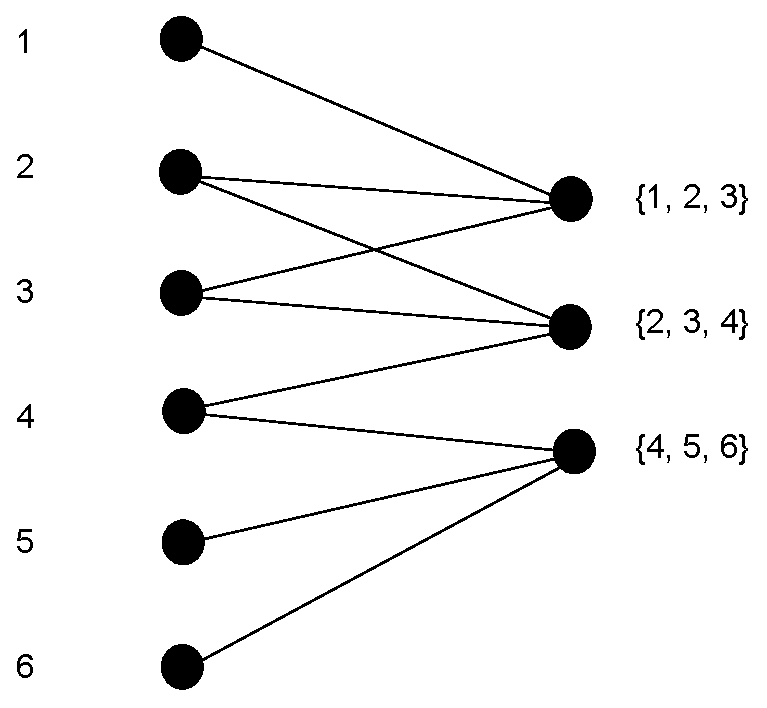
\includegraphics[width=6cm]{Test1/Problem11/deltaA.eps}
                \end{figure}
        
        \item   Geometric representation for $M[\c{A}]$
    \end{enumerate}

\end{proof}